\documentclass{article}
\usepackage[utf8]{inputenc}
\usepackage{geometry}
\usepackage{graphicx} % For including images
\usepackage{hyperref} % For hyperlinks
\usepackage{enumitem}
\usepackage{graphicx}
\usepackage{booktabs} % For professional looking tables
\usepackage{float} % For improved control over floating environments

\geometry{
 a4paper,
 total={170mm,257mm},
 left=20mm,
 top=20mm,
}

\title{Laboratory Assignment 2: Blockchain for Zillow}
\author{Can Acay}
\date{\today}

\begin{document}

\maketitle
\newpage

\tableofcontents
\newpage

\section{Introduction}
This report explores the applicability of blockchain technology to the Zillow real estate platform. It evaluates how blockchain can enhance the functionality and security of Zillow's lease agreement management system and analyzes the impact of such integration on development and deployment.

\section{Software System Selection}
Zillow is an online real estate database company that facilitates the browsing, buying, selling, and renting of homes. It is chosen for this assignment due to its potential for integrating blockchain technology into its operations.

\section{Blockchain Suitability Analysis}

\subsection{Suitable Applications for Blockchain}

\subsubsection{Lease Agreements and Transactions (Chosen module for the analysis)}
Blockchain technology can automate and secure lease agreements and transactions for real estate platforms like Zillow through the use of smart contracts. These contracts facilitate the enforcement of lease terms and the execution of transactions once predefined conditions are met, providing an immutable record that enhances security and trust. This approach simplifies the process, potentially reducing the time and administrative burden associated with traditional methods. Moreover, blockchain's decentralized nature ensures that all transaction records are transparent and resistant to fraud.

\subsubsection{Decentralized Listing and Rating System}
Implementing a decentralized listing and rating system on a blockchain can improve the integrity and reliability of property information on Zillow. By making property listings and reviews tamper-proof and easily verifiable, the system encourages accuracy and honesty in the information provided. This ensures that users have access to reliable data when making decisions, fostering a more transparent environment for property evaluation and selection.

\subsection{Not Suitable Applications for Blockchain}

\subsubsection{Image and Media Storage}
Blockchain technology is not optimal for storing large volumes of images and videos due to its storage cost and size limitations. Real estate platforms like Zillow require efficient, scalable solutions for managing extensive image and video data to showcase properties effectively. Traditional cloud storage services are more suited to this task, offering the necessary scalability and flexibility at a lower cost, thus ensuring that the platform can manage and update its visual content efficiently.

\subsubsection{Real-Time Chat and Communication}
The real-time chat functionality essential for interaction between buyers, sellers, and agents on Zillow demands immediate, high-throughput communication capabilities that blockchain technology cannot provide. The inherent latency in blockchain's transaction processing and the associated costs make it unsuitable for facilitating instant messaging. Alternative web technologies offer the necessary performance, enabling efficient and effective communication without the limitations imposed by blockchain.

\section{Blockchain Category Selection for Lease Agreements and Transactions}
For the module focused on \textbf{Lease Agreements and Transactions} within Zillow, the identified blockchain category is a \textbf{Private, Permissioned Blockchain}.

\section*{Rationale}

The rationale draws upon the decision flowchart provided (Figure \ref{fig:blockchain_decision}), which clarifies the suitability of a blockchain solution.

\begin{figure}[H]
    \centering
    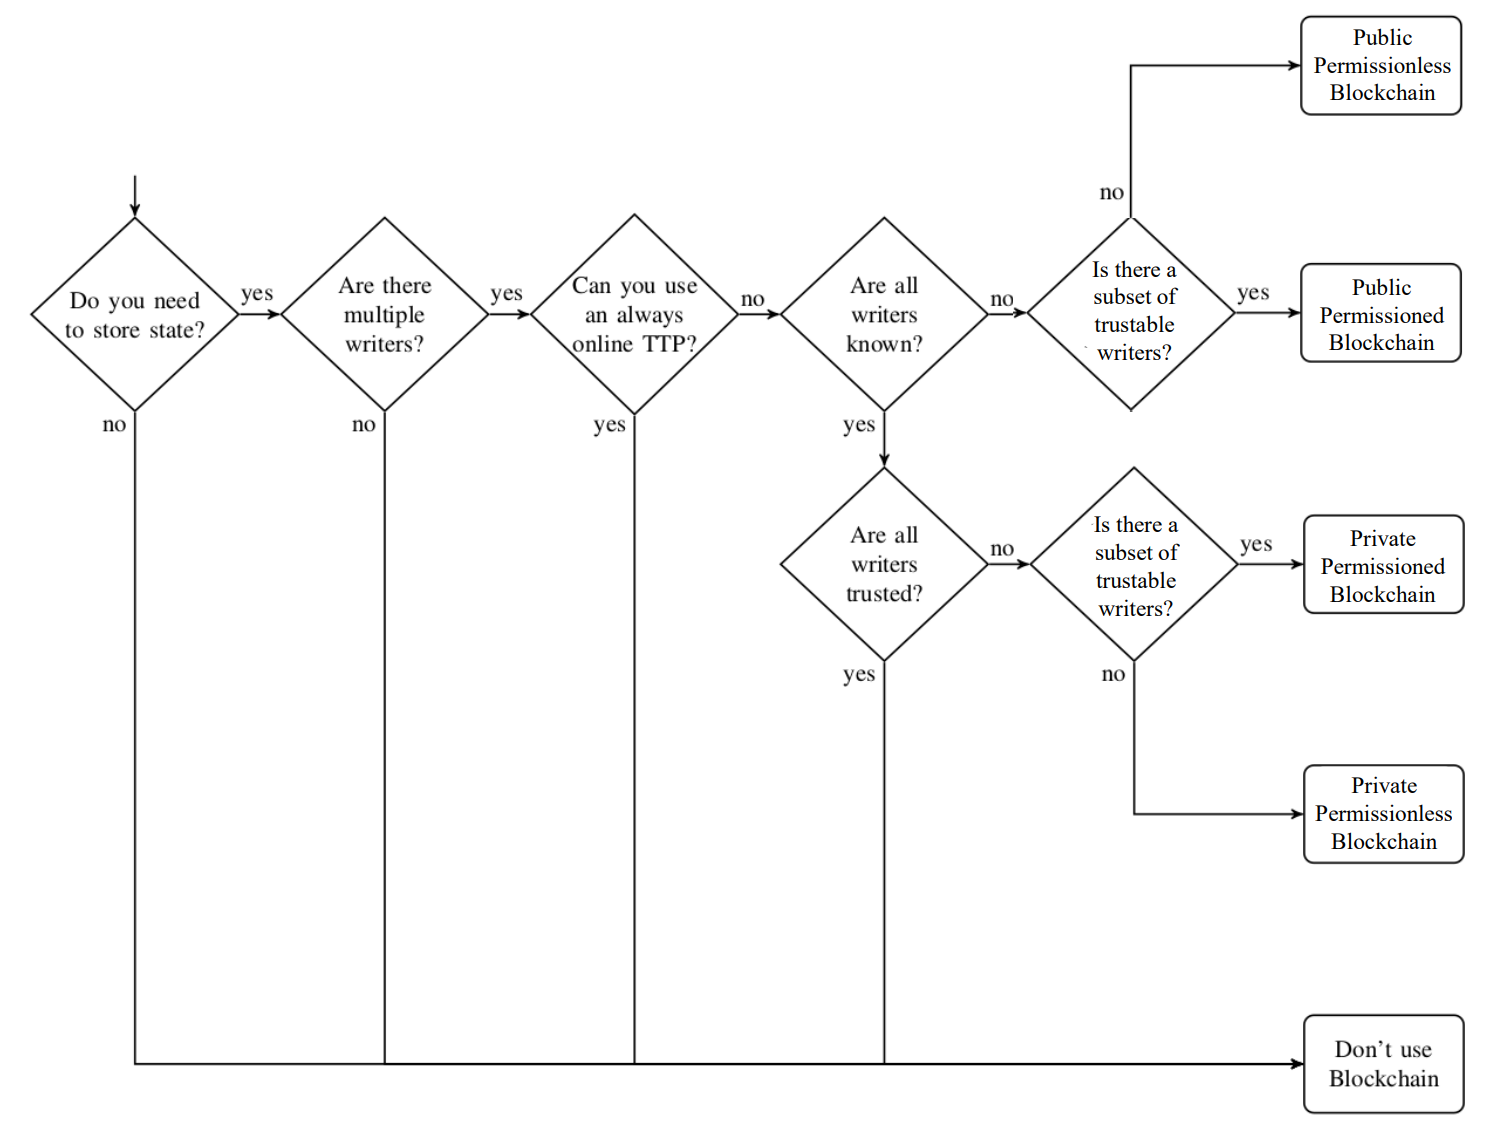
\includegraphics[width=0.8\textwidth]{decisiondiagram.png}
    \caption{Decision flowchart for blockchain applicability.}
    \label{fig:blockchain_decision}
\end{figure}

\begin{itemize}
    \item \textbf{State Storage:} Yes, it is imperative to store the state to maintain current and historical data of leases and sales transactions.
    
    \item \textbf{Multiple Writers:} Yes, the ledger would have multiple contributors, including property owners, tenants, and regulatory entities.
    
    \item \textbf{Trusted Third Party (TTP) Usage:} A decentralized system that reduces dependence on a central TTP is preferable, enhancing trust through the protocol.
    
    \item \textbf{Writer Identity:} All participants in the transaction process on Zillow are identifiable and verifiable, ensuring accountability.
    
    \item \textbf{Writer Trust:} Given the variety of stakeholders with diverse interests, not all writers are inherently trusted.
    
    \item \textbf{Trustable Writers Subset:} A private, permissioned blockchain facilitates a system where a select group of verified participants are granted transaction privileges.
\end{itemize}

The chosen blockchain architecture allows for controlled transaction and viewing capabilities for authenticated users, and participatory consensus among all nodes, which is critical for maintaining integrity and consistency in Zillow's operational model.

\begin{itemize}
    \item \textbf{Transaction and Viewing Rights:} Limited to authenticated users, such as verified property owners, tenants, and administrators, who are authorized to conduct transactions and view lease details.
    
    \item \textbf{Consensus Participation:} Ensuring all changes are collectively validated upholds the ledger's integrity, an essential feature for transaction records in real estate dealings.
\end{itemize}

This approach harnesses the core benefits of blockchain—immutability, traceability, and security—appropriately tailoring the technology to meet the regulatory and privacy demands of real estate transactions.

\section{Design of Smart Contracts and Tokens}

For the lease agreements and transactions module within Zillow, smart contracts and tokens play pivotal roles in streamlining operations and ensuring transaction integrity.

\subsection{Smart Contracts for Lease Management}
Smart contracts will encode lease agreements with pertinent details such as property identifiers, involved parties, payment terms, and conditions of the lease. Operations managed by these smart contracts include:
\begin{enumerate}
  \item Initiation and termination of lease agreements upon consensus of involved parties.
  \item Automated handling of periodic rent payments and issuance of digital receipts.
  \item Management of security deposits and automated enforcement of related terms.
  \item Application of penalties in cases of contract breaches.
  \item Notifications and reminders related to contract milestones.
\end{enumerate}

Smart contracts offer an automated, transparent, and conflict-minimizing approach, which is particularly beneficial for property lease management, addressing the need for a trusted and efficient system.

\subsection{Tokenization in Lease Agreements}
The lease management system will utilize two types of tokens:

\paragraph{Rent Tokens (Fungible):} These tokens represent the monetary value equivalent to the rent payments. They are standardized and carry data including lease identifiers and timestamps.

\paragraph{Security Deposit Tokens (Non-Fungible or Semi-Fungible):} Unique to each agreement, these tokens encapsulate the value and terms of security deposits, acting as proof of commitment held in a digital escrow.

\subsection{Token Lifecycle}
\begin{enumerate}
  \item \textbf{Rent Tokens:}
  \begin{itemize}
    \item Creation upon initiation of a rent payment.
    \item Transfer to the landlord's wallet when the tenant makes the payment.
    \item Redemption or expiration post the rental period, providing an immutable record of the transaction.
  \end{itemize}
  \item \textbf{Security Deposit Tokens:}
  \begin{itemize}
    \item Issuance at the commencement of the lease.
    \item Held in escrow, with terms encoded in the associated smart contract.
    \item Released or forfeited based on the smart contract's resolution upon lease termination.
  \end{itemize}
\end{enumerate}

These token mechanisms ensure a clear, trackable, and enforceable system that aligns with the transparency and security attributes of blockchain technology.

\section{Report on Blockchain Implementation Analysis}

This section presents a detailed analysis of the proposed blockchain implementation for Zillow's Lease Agreements and Transactions module. It outlines the benefits of adopting blockchain technology, the rationale for selecting a specific blockchain category, and the strategic design of smart contracts and tokens, aiming for a comprehensive understanding of blockchain's potential impact on Zillow's operations.

\subsection{Benefits of Blockchain for Lease Agreements and Transactions}
Blockchain technology provides several key advantages for managing lease agreements and transactions on Zillow:

\begin{itemize}
    \item \textbf{Automated Agreement Execution:} Through smart contracts, blockchain facilitates the automatic execution of lease agreements, significantly reducing the need for manual intervention and minimizing disputes.
    \item \textbf{Immutable Transaction Records:} Blockchain ensures the immutability of transaction records, enhancing security and preventing fraud by making it impossible to alter recorded transactions.
    \item \textbf{Transparency and Decentralized Audit Trails:} The technology offers transparency in transactions, providing a decentralized audit trail that benefits users and supports regulatory compliance and oversight.
    \item \textbf{Operational Efficiency:} The adoption of blockchain can streamline processes, potentially reducing the time and administrative burden associated with traditional lease management methods.
\end{itemize}

\subsection{Blockchain Category Rationale}
The selection of a Private, Permissioned Blockchain is based on a thorough analysis tailored to Zillow's specific needs:

\begin{itemize}
    \item \textbf{Privacy and Access Control:} This blockchain type is ideal for handling the sensitive nature of real estate transactions, allowing for robust management of access controls and privacy.
    \item \textbf{Authorized Transactions:} It permits transactions and access to information by authorized entities, such as property owners, tenants, and Zillow administrators, ensuring a secure and controlled environment.
    \item \textbf{Network Integrity and Consistency:} Leveraging the consensus mechanism within a private, permissioned setting maintains the network's integrity and consistency, crucial for real estate dealings.
\end{itemize}

\subsection{Smart Contract Design}
The design of smart contracts for lease management is focused on encoding the complex terms of lease agreements and automating various operations:

\begin{itemize}
    \item \textbf{Terms and Conditions:} Contracts include detailed information such as property identifiers, parties involved, payment terms, and lease conditions.
    \item \textbf{Lease Lifecycle Management:} From the initiation to the termination of leases, smart contracts automate rent collections, manage security deposits, enforce penalties, and send reminders for renewals and due dates.
    \item \textbf{Conflict Reduction:} By automating and encoding lease terms, smart contracts aim to reduce potential conflicts inherent in lease management, offering a transparent and efficient solution.
\end{itemize}

\subsection{Token Design and Lifecycle}
Two types of tokens are implemented to streamline transactions and ensure the integrity of security deposits:

\begin{itemize}
    \item \textbf{Rent Tokens (Fungible):} These tokens standardize rental payments, facilitating efficient and traceable transactions within the system.
    \item \textbf{Security Deposit Tokens (Non-Fungible or Semi-Fungible):} Serve as digital proof of security deposits, with terms encoded in smart contracts, enhancing security and trust in escrow processes.
    \item \textbf{Lifecycle Management:} The process for managing the lifecycle of tokens—from creation to transfer, and ultimately to redemption or release—is clearly defined, ensuring a transparent and auditable system.
\end{itemize}

\subsection{Conclusion}
Integrating blockchain technology into Zillow's Lease Agreements and Transactions module is expected to significantly enhance the platform's security, efficiency, and transparency.

\end{document}
